
\chapter{Conceitos Básicos de Sintese de Voz}
\section{Anatomia da Voz}
	Para estudar a produção e a síntese da voz, é necessário ter um conhecimento acerca da anatomia e do funcionamento físico da voz~\cite{Foundation1}. Sendo assim, as subseções seguintes descreverão brevemente detalhes da anatomia do sistema fonador humano e como o som é produzido, moldado e influenciado por este sistema.
	\subsection{A Anatomia}
	A Figura~\ref{fig:aparelhoFonador}~\cite{Foundation1}, mostra os órgãos associados com a produção da voz. Dentro das condições normais, a voz é produzida quando um fluxo de ar vindo dos pulmões é convertido em energia acústica através da vibração das pregas vocais, localizadas na laringe. Os padrões de vibrações resultantes são moldados acusticamente quando o som passa pelo trato vocal acima da laringe. O sistema respiratório serve como uma
	
	\begin{figure}
		\centering
		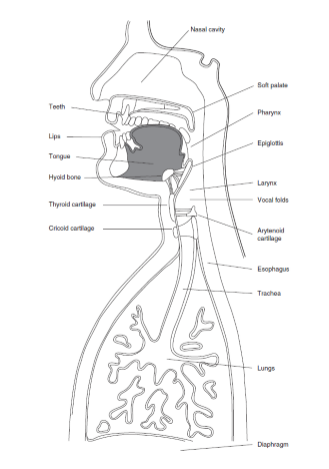
\includegraphics[scale=0.5]{aparelhoFonador}
		\caption{Aparelho Fonador}
		\label{fig:aparelhoFonador}
	\end{figure}
	
	fonte de potência para a produção do som, sendo responsável por movimentar o ar através do trato vocal. A laringe atua como um oscilador convertendo a potência aerodinâmica produzida em energia sonora, sendo frequentemente retratada como a fonte da voz. No entanto, a mais importante função da laringe não é a produção de som, e sim, vedar as vias aéreas aos pulmões completamente, protegendo-as de objetos estranhos ou líquidos, principalmente durante a deglutinação. De maneira análoga, a laringe serve como uma válvula de acesso às vias respiratórias e por essa característica, atua também no controle do fluxo de ar que por elas passam. Sendo assim,é fácil notar que há uma necessidade de mobilidade para toda estruturada laringe, logo é de se esperar que sua estrutura seja formada em sua maioria por cartilagens. De fato o é, com exceção de um osso chamado de Hioide, a laringe é basicamente formada por cartilagens e músculos. A seguir, analisaremos brevemente a dinâmica dos músculos e cartilagens da laringe.
	\subsection{Músculos e Cartilagens}
	Os músculos e cartilagens atuam diretamente no processo de abdução e adução das pregas vocais. Estas estão localizadas dentro da laringe e devido à dinâmica das cartilagens e dos músculos, podem executar os movimentos citados de forma a produzir som.
	
	\subsubsection{Cartilagens da Laringe}

	
	\begin{figure}
		\centering
		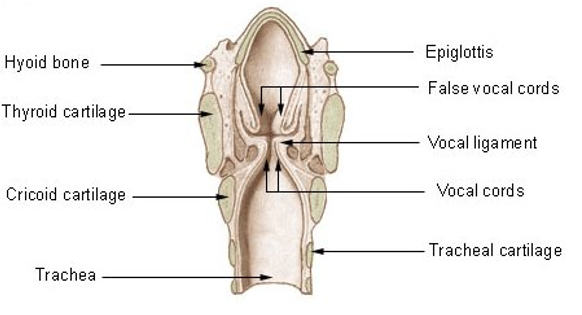
\includegraphics[scale=0.5]{cartilagensLaringe}
		\caption{: Secção coronal da laringe e parte superior da traquéia.~\cite{Foundation1}}
		\label{fig:aparelhoFonador}
	\end{figure}
	
	De maneira sucinta, estas cartilagens servem como base de interconexão para os músculos intrínsecos ao redor da laringe. Dentre as cartilagens acima, a epiglote é responsável por vedar as vias respiratórias movimentando-se sobre a entrada das mesmas. O resto das cartilagens garantem a mobilidade da laringe em conjunto com outras estruturas como por exemplo o sternum.
	
	Os músculos na laringe podem ser divididos em dois grupos, os intrínsecos e os extrínsecos [1]. Os músculos intrínsecos interconectam as cartilagens da laringe, ao passo que, os extrínsecos conectam a laringe à outras estruturas externas, como o osso hióide. A Figura ~\ref{fig:musculosLaringe} detalha alguns dos músculos intrínsecos da laringe. Alguns desses músculos têm influência direta em algumas características da voz. Por exemplo, o músculo cricotiroideo é o músculo primário utilizado no controle do tom da voz. Por sua vez, o músculo cricoaritenoideo posterior atua na abdução das pregas vocais, ao passo que o músculo interaritenoideo atua como adutor das pregas vocais.
	
	\begin{figure}
		\centering
		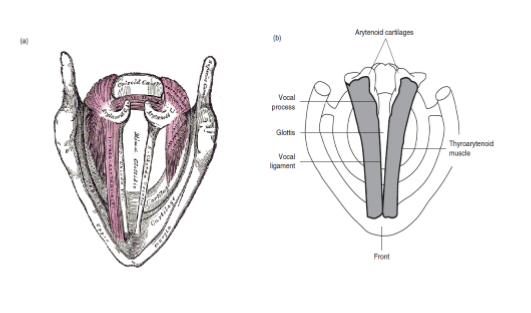
\includegraphics[scale=0.5]{musculosLaringe}
		\caption{: Músculos Intrínsecos da Laringe.~\cite{Bell}}
		\label{fig:musculosLaringe}
	\end{figure}
	
	Os músculos extrínsecos, Figura ~\ref{fig:musculosLaringe}, atuam basicamente no movimento da laringe, agindo como depressor e elevador da estrutura laríngea. Além disso também conectam estruturas do trato vocal à estrutura laríngea, como por exemplo a língua ao osso hioide.
	
	\begin{figure}
		\centering
		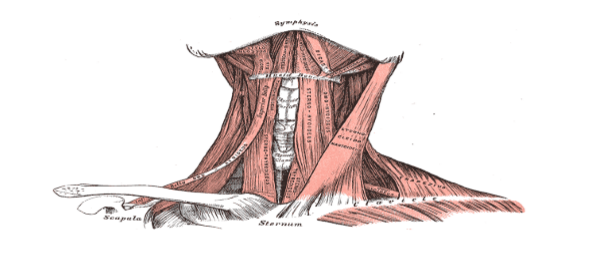
\includegraphics[scale=0.5]{musculosPescoco}
		\caption{:Músculos Extrínsecos da Laringe.~\cite{Bell}}
		\label{fig:musculosPescoco}
	\end{figure}	
	
	\subsection{Pregas Vocais}
	As pregas vocais, como dito anteriormente, estão localizadas dentro da laringe, mais especificamente na parte superior da traqueia. Elas estão posteriormente ligadas às cartilagens aritenoides, e anteriormente ligadas à cartilagem tireoide. As suas bordas exteriores estão ligadas a músculos na laringe, enquanto as suas bordas interiores são livres.
	
	As bordas das pregas vocais são construídas de epitélio, sendo compostas também de algumas fibras musculares. As pregas vocais são bandas triangulares planas de cor branca e acima de ambos os lados destas, se encontram as pregas vestibulares ou falsas pregas vocais. O espaço entre as pregas vocais é chamado de glote, sendo que o que está acima da glote é denominado supraglotal e o que está abaixo é denominado subglotal. A Figura~\ref{fig:cordasVocais} mostra em mais detalhes a anatomia das pregas vocais, os componentes musculares e as cartilagens atuantes.
	
	\begin{figure}
		\centering
		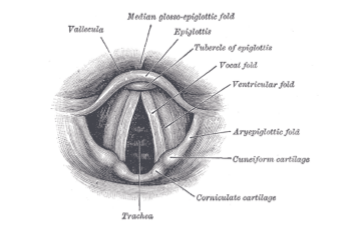
\includegraphics[scale=0.5]{cordasVocais}
		\caption{:Cordas Vocais e Componente~\cite{Bell}}
		\label{fig:cordasVocais}
	\end{figure}	
	
	\subsection{Overview: Geração de Som e Ressonadores}
	
	A produção do som da voz é composta de duas etapas importantes que ocorrem na região subglotal/glotal e supraglotal. A primeira é a transformação da energia aerodinâmica em energia sonora, pelo movimento e vibração das pregas vocais.
	
	O segundo é a transformação do som primitivo gerado em voz, através da atuação dos ressonadores e formantes na região supraglotal.
	
	A vibração das pregas vocais é extremamente complexa e, diversos músculos em união com a pressão exercida pelo ar atuam para tornar esse movimento possível. De maneira sintetizada, as pregas vocais vibram do topo ao fundo de maneira que não vibram como se fosse um bloco, mas sim de forma ondulatória, conforme mostrada na Figura~\ref{fig:movimentoCordas}. Essa vibração é responsável por mudanças depressão entre a região subglotal e a região glotal, causando uma diferença de pressão(condensação e rarefação) nessa área durante o movimento das pregas vocais, o que ocasiona a geração de som.

	\begin{figure}
		\centering
		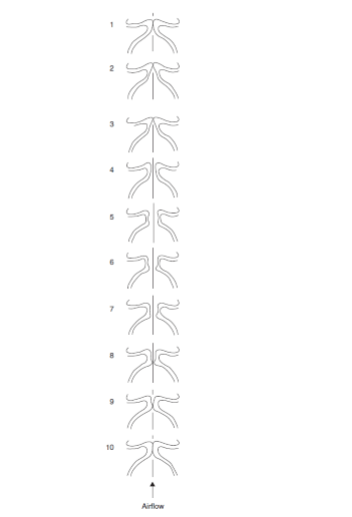
\includegraphics[scale=0.5]{movimentoCordas}
		\caption{:Movimento das Cordas Vocais ~\cite{Foundation1}}
		\label{fig:movimentoCordas}
	\end{figure}		
	
	Entretanto, o som produzido é um som primitivo, conforme dito anteriormente, e para se transformar na voz característica humana, ele deve ser filtrado e moldado pelos ressonadores(formantes) no trato vocal(Figura ~\ref{fig:tratoVocal}).
	Todas as cavidades mostradas no trato vocal atuam como ressonadores para a onda sonora produzida pelas pregas vocais. Um ressonador pode entrar em estado de vibração através de uma força aplicada ao mesmo em inércia ou por interação com algo que já esteja em estado de vibração.
	
	Neste segundo caso, as vibrações produzidas pelo ressonador serão amplificações ou atenuações dependendo de quão próximas ou distantes, em termos de frequência, são as vibrações da onda sonora em contato com o ressonador. Caso a onda sonora possua vibrações cujas frequências se assemelhem às frequências do ressonador,estas então serão amplificadas pelo ressonador.
	
	Entretanto,caso as frequências do som gerado vibrem em uma frequência distante da frequência natural do ressonador, então estas serão abafadas. A voz passa por esse processo ao ser formada. Um som primitivo advindo das pregas vocais entra em contato com os ressonadores no trato vocal, estes por sua vez em conjunto

	\begin{figure}
		\centering
		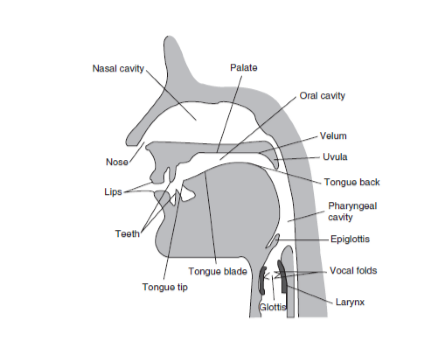
\includegraphics[scale=0.5]{tratoVocal}
		\caption{:Trato Vocal~\cite{Foundation1}}
		\label{fig:tratoVocal}
	\end{figure}		
	

	Os conceitos e propriedades descritos acima são extremamente importantes para se entender a manutenção da produção do som. As pregas vocais são músculos e músculos são compostos por fibras, logo, as pregas vocais consistem de uma grande concentração de fibras. Além disso, entre as fibras que compõe as pregas vocais existem também fluidos atuantes, o que caracteriza as pregas vocais como um material viscoelástico.
	
	Para se entender a capacidade de absorção e regeneração das pregas vocais, em detrimento das vibrações de alta frequência e as pressões do ar, deve-se primeiramente estudar as propriedades absorcivas do material que as compõe. Ou seja, em outras palavras, deve-se estudar as propriedades mecânicas do tecido viscoelástico, e uma ferramenta que facilita o entendimento é o estudo da curva força-alongamento de um material. Entretanto, construir uma curva de força-alongamento depende essencialmente da geometria da amostra do material~\cite{IngoTitze} e, por se tratar de uma material biológico, é difícil obter uma geometria precisa pois as fibras estão constantemente se reorientando em detrimento de lesões e cortes fibrosos. Para viabilizar este estudo, Titze~\cite{IngoTitze} sugere normalizar as forças atuantes e as deformações resultantes para que não haja a dependência direta da geometria. Essa normalização se dá através da substituição da curva força-alongamento por um curva tensão-deformação. A Figura ~\ref{fig:curvaTensao} retirada do estudo feito por Titze ~\cite{IngoTitze} demonstra uma curva hipotética de tensão-deformação para os tecidos que compõe as pregas vocais humanas. 
	
	Esta Figura ilustra o comportamento das fibras das pregas vocais através da relação entre uma força atuante e a deformação gerada por esta.
	 A importância desta analises e deve ao fato de que é possível estabelecer uma relação direta entre nódulos vocais e uma fonação prolongada, alta(em termos de frequência) e intensa. A partir da análise desta curva é então possível estabelecer um precedente para a formação de nódulos vocais: a frequência e amplitude da vibração estão diretamente ligadas ao surgimento de um nódulo vocal e consequentemente o de uma fenda pois a força de impacto entre as pregas vocais é proporcional à altura tonal quando acima do tom natural e à intensidade durante a fonação.
	
	\begin{figure}
		\centering		
		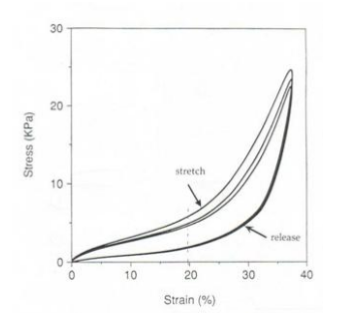
\includegraphics{figura1.png}
		\caption{:Curva Hipotética Tensão-Deformação das Cordas vocais Humanas~\cite{IngoTitze}}
		\label{fig:curvaTensao}
	\end{figure}
	
	
